\section{Data Cache}
This section describes the structure of the data cache and its role in the memory system.

\subsection{Brief Overview}

The data cache is a writeback, 2 way associative cache. 
The cache uses physical tagging and virtual indexing, so the number of bytes in each way is limited to the size of a tiny translation page (1024 bytes). 
The default cache size is $64 \text{ lines} \cdot 4 \text{ words/line} \cdot 4 \text{ bytes/word} = 1024 \text{ bytes}$. 
The number of lines per way is parameterized, and the replacement policy implemented is Least Recently Used (LRU).

\subsection{Important Diagrams}

	Figure \ref{fig:dcachediag} includes a diagram of the data cache.
	See the code for more information.
	\begin{figure}
	\label{fig:dcachediag}
	\centering
	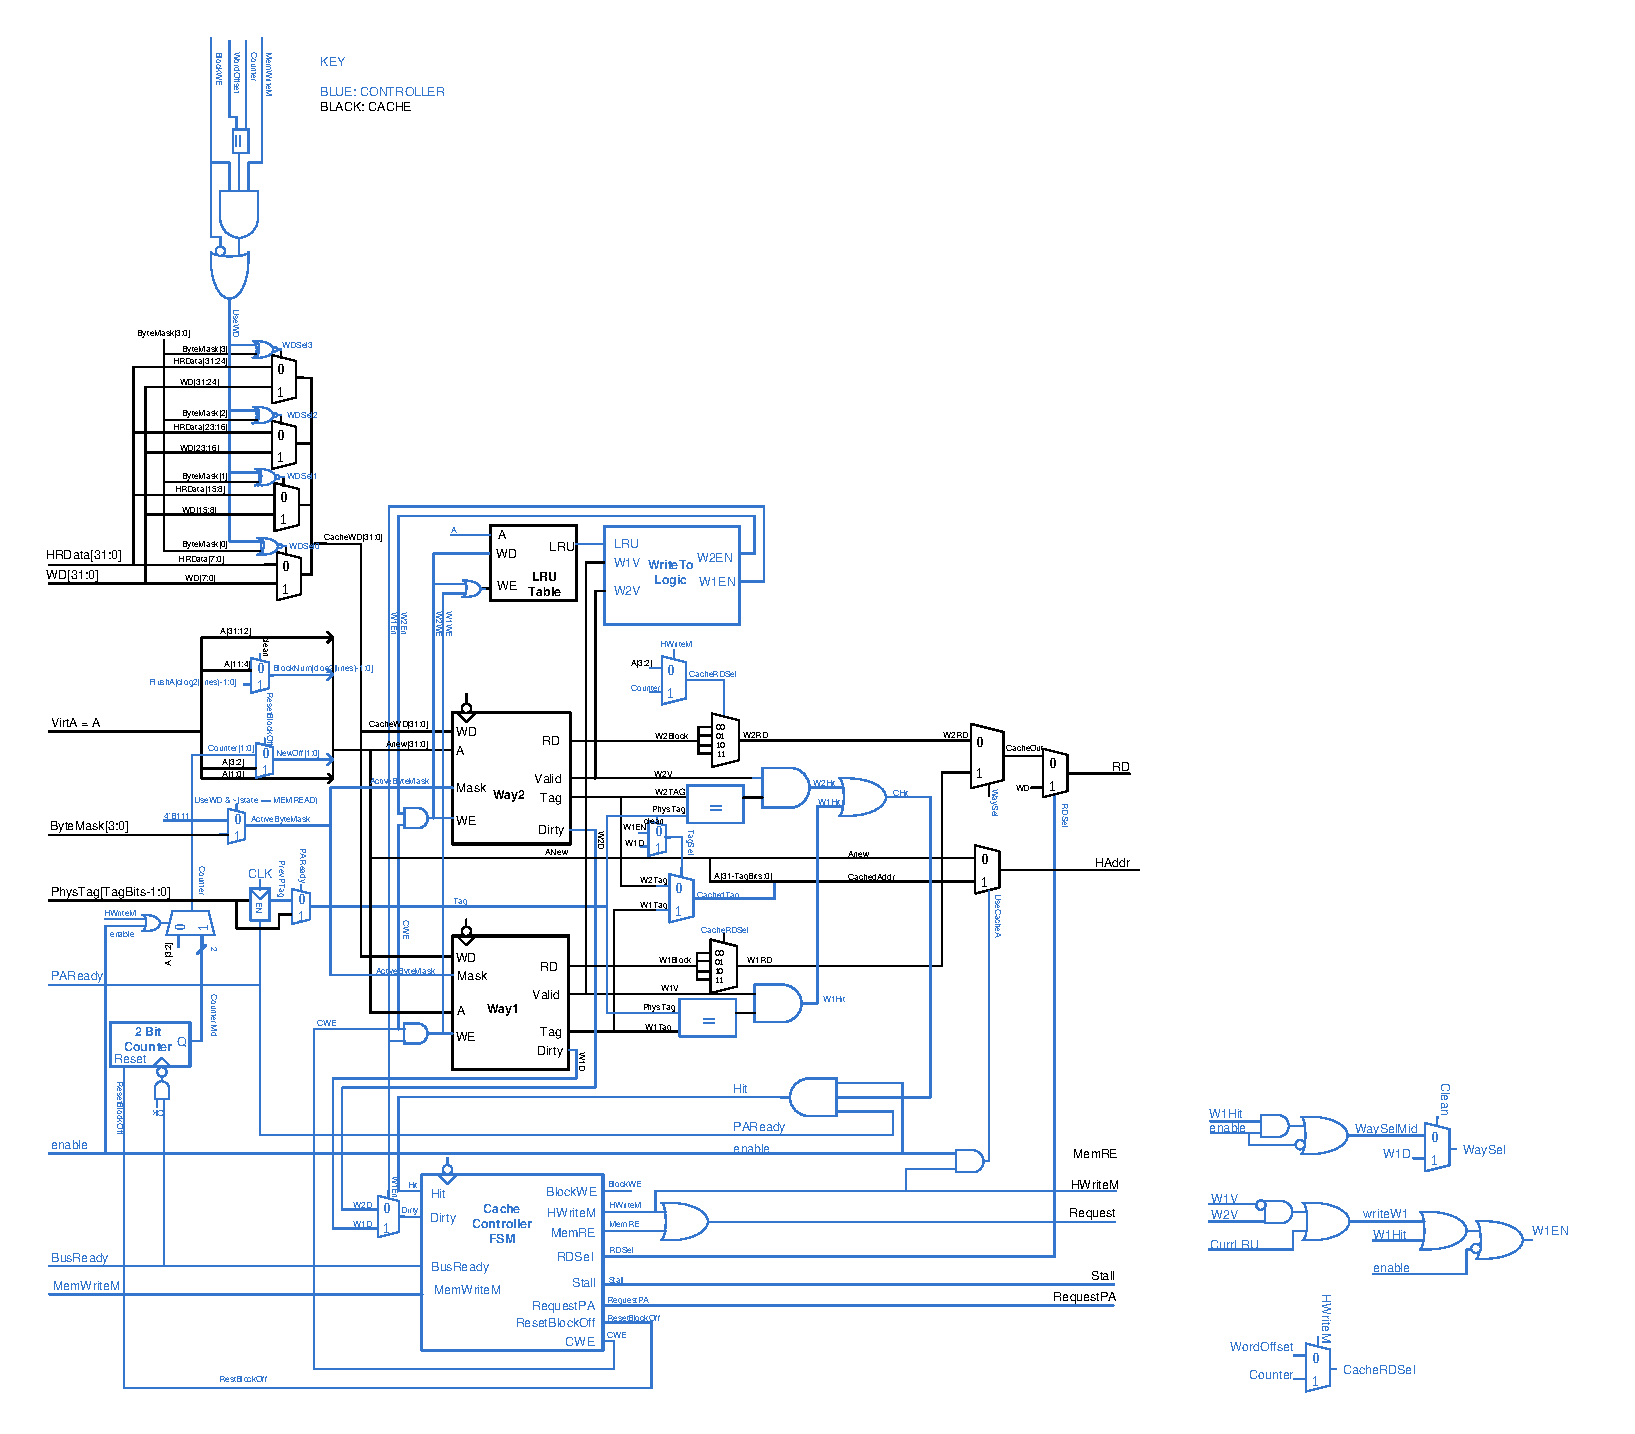
\includegraphics[width=\textwidth]{images/dataCache.pdf}
	\caption{Diagram of 2 way set associative data cache. Controller logic in blue}
	\end{figure}

\subsection{All Relevant Files and Brief Descriptions}

	Table \ref{table:drel} shows the files that are used by the data cache and Table \ref{table:dio} lists the top level inputs and outputs.

	\begin{table}
	\label{table:drel}
	\begin{tabular}{|l|p{70mm}|}
	\hline File  & Description \\ 
	\hline  data\_writeback\_associative\_cache.sv & Top level D\$ module \\ 
	\hline  data\_writeback\_controller.sv & Controller logic for the D\$.
	Contains the primary state machine described in section \ref{sec:dstate} \\ 
	\hline  data\_writeback\_associative\_memory.sv & 
	Memory module containing the both cache ways, the LRU memory, and way selection mux's.
	This module is used in both the instruction and data caches.
	The instruction cache fixes the dirty and clean inputs to zero, because it is a read only cache.\\ 
	\hline  data\_writeback\_associative\_cache\_way.sv & 
	Contains the memory associated with one cache way. This includes four words per line along with the valid, dirty, and tag bits. \\ 
	\hline  word\_memory.sv & Byte addressable word memory  \\
	\hline
	\end{tabular} 
	\caption{Data cache files}
	\end{table}

	\begin{table}
	\label{table:dio}
	\begin{tabular}{|l|p{85mm}|l|}
	\hline Port & Description & I/O \\ 
	\hline clk & Clock input &  I \\ 
	\hline reset & Global reset signal &  I \\ 
	\hline MemWriteM & Write signal from datapath &  I \\ 
	\hline MemtoRegM & Read signal from datapah & I \\ 
	\hline IStall & Instruction cache stall. Used to avoid multiple data acesses for the same instruction & I \\
	\hline VirtA[31:0] & Virtual address from the leg datapath & I \\
	\hline WD[31:0] & Write data from LEG datapath & I \\
	\hline CP15en & Enable signal from the coprocessor & I \\
	\hline Inv & Invalidate line signal from the coprocessor & I \\
	\hline AddrOp & Indicates coprocessor is invalidating or cleaning using a virtual address instead of a set index. When high, only clean or invalidate on a hit in the data cache.& I \\
	\hline InvAllMid & When InvAllMid and Inv are high, invalidate all lines from cache. This signal is driven by the coprocessor & I \\
	\hline CurrCBit & Cachable bit for the current TLB entry & I \\
	\hline PAReady & Indicates TLB entry is valid for the data cache. The data cache uses the physical address and control bits from the TLB & I \\
	\hline PhysTag[tbits-1:0] & Physical Tag from the TLB & I \\
	\hline ByteMaskM[3:0] & ByteMask from leg controller & I \\
	\hline HRData[31:0] & Data from the AHB Bus & I \\
	\hline BusReady & AHB Ready signal & I \\
	\hline MSel & Indicates data cache has control of the AHB Bus & I \\
	\hline Stall & Stall signal from the data cache controller & O \\
	\hline RequestPA & Request a physical address from the TLB & O \\
	\hline HWData[31:0] & AHB Write data & O \\
	\hline RD[31:0] & Data output from the cache. This is the same as HWData. & O \\
	\hline HAddr[31:0] & AHB write address & O \\
	\hline HSizeM & AHB write size & O \\
	\hline HRequestM & Request AHB control & O \\
	\hline HWriteM & AHB write enable & O \\
	\hline
	\end{tabular} 
	\caption{Data cache I/O (data\_writeback\_associative\_cache.sv)}
	\end{table}
	% TODO: Fix the label and reference

\subsection{Data Cache States}
\label{sec:dstate}

Below is an explanation of the data cache states.

\begin{enumerate}
	\item READY 
	The ready state is the default state for the data cache.
	Upon a cache hit, the data cache will remain in the READY state.

	\item WRITEBACK
	The cache enters the writeback state to writeback each word from the line to memory.
	If the data cache attempts to replace a dirty line, then it is written back first.
	The data cache stays in this state for at least three cycles to writeback the first three words from the dirty line.

	\item LASTWRITEBACK:
	The last writeback state in the cache. 
	During this state, the data cache does not request a new memory access.
	It waits for the last writeback to complete.

	\item MEMREAD:
	Data cache enters this state on a cache miss to read data from memory.
	The cache reads four words sequentiall from the AHB Bus.

	\item LASTREAD:
	The last memread state in the cache. 
	During this state, the data cache does not request a new memory access.
	It waits for the last memory read to complete.

	\item NEXTINSTR:
	The next instr state removes the stall on the pipeline and allows the instructions to move one stage down the pipeline. If this stage did not exist, then the instruction at the data stage would remain the same and after the requested data is retrieved, the same data would be retrieved again. 

	\item WAIT:
	The data cache enters this state when simultaneous data and instruction stalls occur. 
	The data cache has bus precedence, so after it is done using the bus it waits for the instruction cache to retrieve data before handling the next request. 
	This state avoids repeating data acesses when the processor stalls.

	\item DWRITE:
	This state handles disables full word writes to main memory.
	
\end{enumerate}
